\documentclass[a4paper, titlepage, 10pt]{book}


\usepackage{graphicx}
\usepackage{caption}
\usepackage{amsmath,amssymb}
\usepackage{siunitx}
\usepackage{hyperref}

\usepackage{geometry}
\geometry{a4paper, top=2.5cm, bottom=2.5cm, left=2.4cm, right=2.4cm, heightrounded, bindingoffset=0.2cm}

%migliora l'aspetto delle testatine
\usepackage{emptypage} %toglie testatine da pagine vuote
\usepackage{fancyhdr}
\pagestyle{fancy}
\renewcommand{\chaptermark}[1]{\markboth{#1}{}}
\renewcommand{\sectionmark}[1]{\markright{\thesection\ #1}}
\fancyhf{}
\fancyhead[LE,RO]{\scshape\thepage}
\fancyhead[LO]{\scshape\footnotesize\nouppercase{\rightmark}} 
\fancyhead[RE]{\scshape\footnotesize\nouppercase{\leftmark}}

%comando per l'abstract (non esiste nella classe book)
\newenvironment{abstract}{%
	\newpage\thispagestyle{empty}\vspace*{3\baselineskip}
	\begin{center}\Large\textbf{Abstract}\end{center}%
	\begin{quotation}%
	}{\end{quotation}\clearpage}


\title{The evolution of the night sky spectrum in Asiago}
\author{Marco Codato}
\date{Master Thesis in Astrophysics and Cosmology}

\begin{document}
\maketitle

\thispagestyle{empty}
\
\begin{abstract}
	\addcontentsline{toc}{chapter}{Abstract}
	Modern sky brightness monitoring techniques aim to precisely measure the total amount of radiation from the observing site but very little can be said about the various sources responsible for such radiation.
	In this work I use spectra acquired in the last 15 years from the Asiago Observatory to identify the various sources in the sky and study their temporal evolution.
\end{abstract}

\clearpage

\tableofcontents

\chapter{Introduction}
Part I: Sky sources in theory
\begin{itemize}
	\item Introduction
		\subitem General introduction
		\subitem Aim of the work
		\subitem About the methodologies
	\item The natural sky
		\subitem Main natural sources
		\subitem And their footprint on spectra
	\item The light pollution
		\subitem Definitions and aftermaths
		\subitem Mechanism of working
		\subitem Mention to the models in the literature
		\subitem LP footprint in spectra
\end{itemize}
Part II: Analysis of sky background in spectra
\begin{itemize}
	\item Software description
		\subitem Bkg extraction
		\subitem Bkg analysis
	\item Results
	\item Discussion and interpretation of the results
	\item Conclusions
\end{itemize}

\section{Light pollution}
Light pollution (LP) is the alteration of the natural light level due to artificial sources. The resulting increase of the sky brightness has many proven negative effects.

\paragraph{Effects on the human health.} Light exposure in nigh time decrease the natural production melatonin. The effect is proportional to the frequency of light, with bluer radiation producing a stronger decrease of melatonin production.
	
Melatonin is an important hormone that regulates many biological mechanism. It is capable of prevent some forms of cancer and is responsible of the sleep regulation. A melatonin deficiency has been proven to be correlated with higher chances of developing breast and prostate cancers and a decrease of sleep time and quality, which typically lead to further health disorders.
	
Melatonin decrease is proportional both to light intensity and frequency. A greater effect is given by brighter and bluer sources. In this context the spreading of LED lights, with their strong emissions in the blue side of visible spectrum, is considered a concern by many health associations.

\paragraph{Effects on the environment.} LP affects other living beings as well as humans. Animals exposed to abnormal level of light at night change their behaviour and habits. Note this form of pollution is probably the most widespread but yet one of the least acknowledged.

\paragraph{Economical effects.} When looking at a artificially bright sky one should consider that such photons that brighten the sky are no longer being used for the purpose they were made for, i.e.\ lighten streets, houses, commercial areas and so on. The energy, and thus the cost, to produce such photons is wasted. 

Unluckily in the last years efficient light sources like LEDs allowed to produce powerful lighting systems at low cost making the economical argument less relevant. Since light is cheaper, it is less critical weather part of it is lost toward the sky.

\paragraph{Cultural effects.} All the cultures around the world developed myths and legends involving the heavens; night sky inspired artists and philosophers in western cultures for centuries and in general the observation of a starry sky always belonged to the human experiences. Today due to LP FabbriXX estimates that at least the XX\% of the world population lives in areas where milky way is not even visible and only a handful of bright stars can stand out of the polluted sky. In terms of traditions and human experience this is a great loss, but yet difficult, or impossible, to quantify.

\paragraph{Scientific effects.} Of course the increase of sky brightness made astronomical observations more difficult. Observation sites moved from the town centres in the XIX century to the rural areas due to the introduction of the first lighting. With the growing urbanization, many of these sites ended up to by at the limb of the expanding urban areas, heavily limiting the possibility of relevant scientific activities. Nowadays it is likely that in a country no totally dark sites are available, forcing astronomers to build new instruments in very remote areas in poorly populated areas of the world.

A typical example of the effects in the changing of the sky condition is the Asiago observatory. It was built in 1942 in a poorly populated highland, which also offered an adequate shielding from the light of the yet small rural centres in the nearby pianura veneta. When built, the observatory also hosted the largest reflecting telescope in the Europe (Gaileo telescope, 122\,m of diameter).
With the economic boom in the 50s, industrial and manufacturing activities replaced agriculture in the Veneto flatland. Urban areas significantly expanded making Veneto region one of the most light polluted sites in the whole Europe. At the same time the Asiago highland become one of the most appreciated touristic destination in the surrounding area. The quality of the sky rapidly worsened also with respect to other nearby areas less touched by human activities. In such new condition the Asiago Observatory lost its central role in research activities tough preserving its nature of scientific pole.

\section{Aim of the work}
For all the issues above measuring and monitoring the LP is of crucial important. 

\chapter{The natural sky background}
Even when artificial sources are neglected, there are still several natural background sources. In this chapter each contribution will be described in detail. In the plot on the Figure \ref{fig:natural_sources} are reported, in logarithmic scale, the main background sources for a wide range of wavelengths, from UV to radio emission. In the next lines I will consider only sources relevant for optical observations.
\begin{figure}
	\centering
	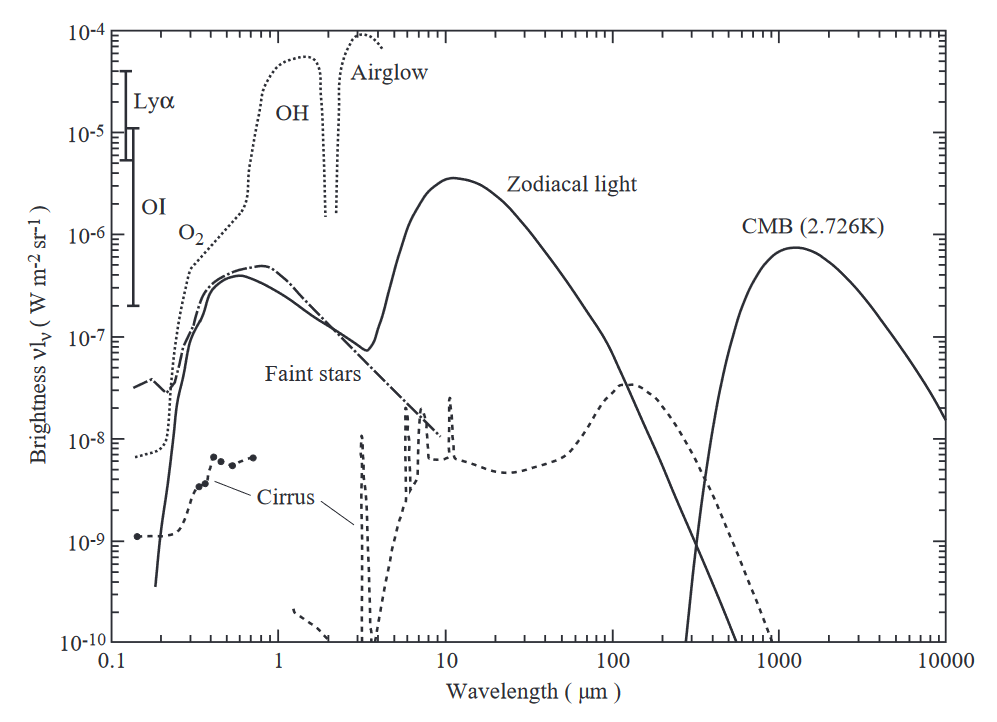
\includegraphics[width=.7\textwidth]{./2_natural_sky/natural_sources}
	\caption{Different sky brightness contributions in different electromagnetic domains. In the optical band most relevant contribution ar Airglow, zodiacal light and faint stars. From \cite{leinert19981997}.\label{fig:natural_sources}}
\end{figure}
For clarity I will distinguish between extraterrestrial sources from the terrestrial or atmospheric ones. At the end of the chapter I will also discuss about the contribution on the sky background due to atmospheric scattering effects.

Quantitatively the total sky brightness can be expressed as
\begin{equation}
	I_\text{sky} = (I_A+I_{ZL}+I_{ISL}+I_{DGL}+I_{EBL})e^{-\tau}+I_\text{sca}
\end{equation}
where A stands for airglow, EZ is zodiacal light, ISL integrated galactic light, DGL diffuse galactic light and EBL extragalactic background light. $\tau$ is the extinction coefficients and $I_\text{sca}$ gathers all the scattering terms, i.e.\ light scattered from previous sources and from light pollution, from \cite{leinert19981997}.


\section{Extraterrestrial sources}
I will first consider sources of photons outside the earth atmosphere. Using space-based instrument it is possible to study these components without the interference of atmospheric emissions.

\subsection{Zodiacal light}
Zodiacal light consists on sunlight scattered by interplanetary dust particles \cite{leinert1975zodiacal}. From the Earth it looks like a white glow visible during the twilight and extending from the Sun in the zodiacal region.
\begin{figure}
	\centering
	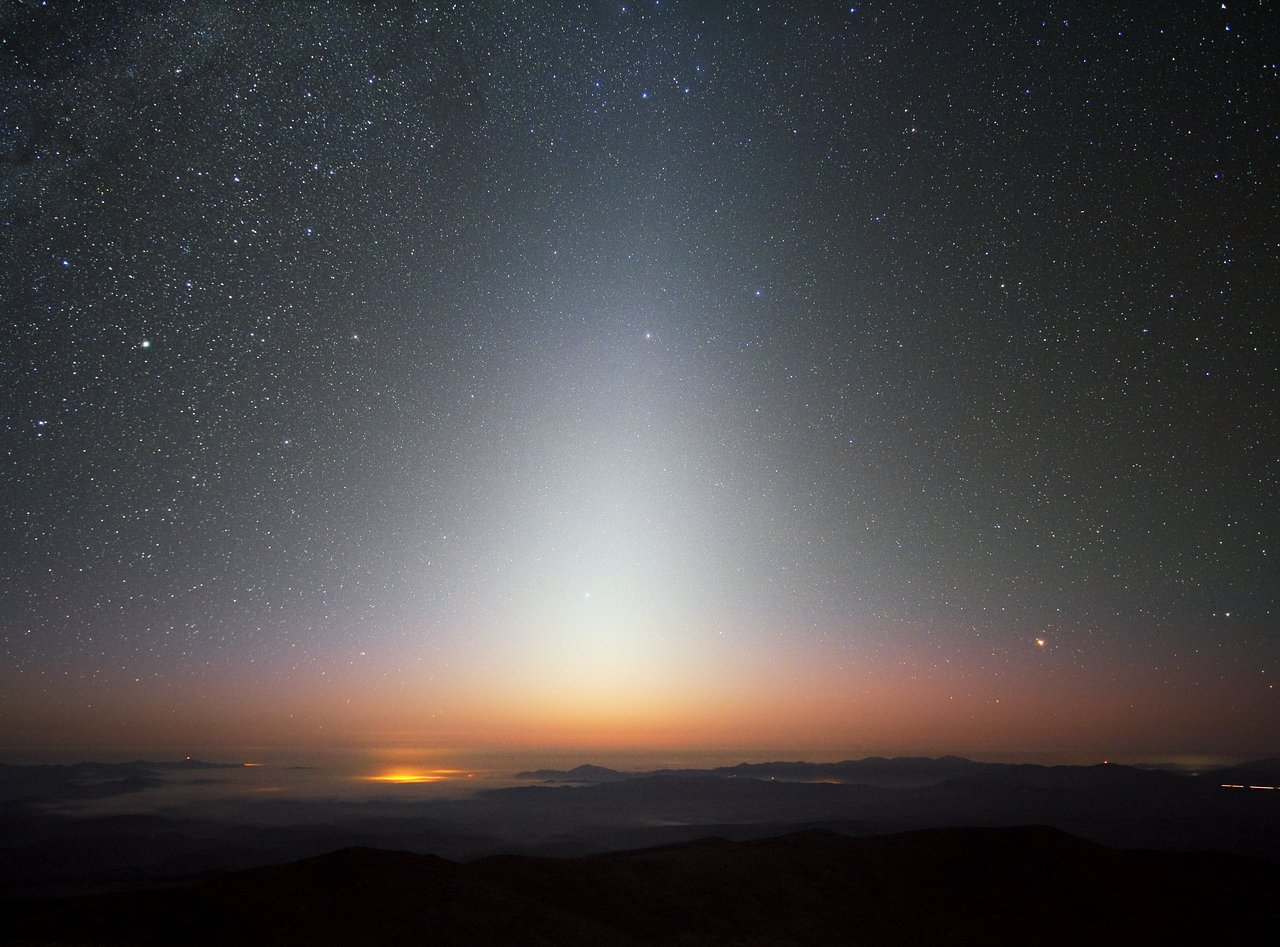
\includegraphics[width=.8\textwidth]{./2_natural_sky/zodiacal_ima}
	\caption{Zodiacal light after sunset at La Silla, Chile. Source: \href{https://www.eso.org/public/images/zodiacal_beletsky_potw/}{eso.org}.\label{fig:zodiacal_ima}}
\end{figure}

\paragraph{Angular distribution.} The figure \ref{fig:zodiacal_distribution}, adapted from \cite{frey1974photometry}, describes the angular distribution of the zodiacal light in ecliptic coordinates. Such light is maximum along the ecliptic and close to the Sun. A fainter local maximum is present in direction opposite to the Sun. It is known as \emph{gegenschein} and is produced by back-scattered solar light. Zodiacal light brightness varies from about \SI{e-6}{erg\per\second \per\centi\metre\squared \per\steradian\per\angstrom} on the ecliptic at \ang{30} from the sun to about \SI{e-9}{erg\per\second \per\centi\metre\squared \per\steradian\per\angstrom}. Gegenschein maximum brightness reaches about \SI{e-7}{erg\per\second \per\centi\metre\squared \per\steradian\per\angstrom}. After the airglow (see \S XX), this is the second brightest background source in optical bands.

\begin{figure}
	\centering
	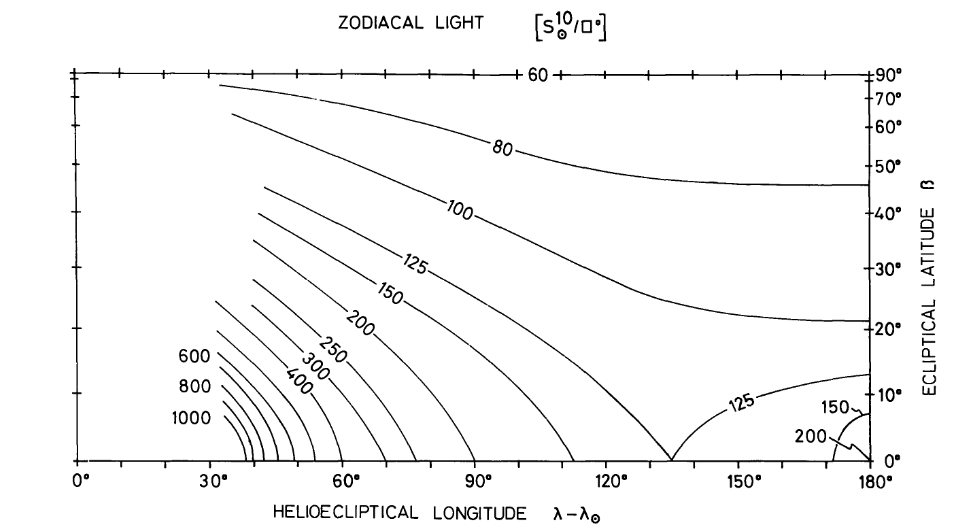
\includegraphics[width=.8\textwidth]{./2_natural_sky/zodiacal_distribution}
	\caption{Isophotal map ot the zodiacal light as \SI{7100}{\angstrom}. As a reference, according to \cite{leinert19981997}, $\SI{1}{S}_{10}/\square^\circ = \SI{9.21e-10}{erg\per\second \per\centi\metre\squared \per\steradian\per\angstrom}$ at those wavelengths. From \cite{frey1974photometry}.\label{fig:zodiacal_distribution}}
\end{figure}

The contribution of zodiacal light to the optical background is maximum during the twilight, after sunset in spring or before sunrise in autumn, from the northern hemisphere.

\paragraph{Spectral energy distribution.} Being essentially reflected sunlight, the optical zodiacal light energy distribution has the same shape of the solar one.

\subsection{Galactic background}
In optical bands a significant contribution to the background level is provided by unresolved stars in the Galaxy. The contribution of such sources depends on the ability of resolve the brightest stars \cite{leinert19981997}, i.e.\ on the limiting magnitude of the instrument.

\paragraph{Angular distribution.} Unresolved stars background follows the morphological structure of the Milky Way. The signal is higher toward the galactic plane and the galactic center.  Its spectrum follows typical optical stellar spectra with the characteristic black-body emission. It is the third most relevant contribution to the optic continuum with an emission that spans from peak values of \SI{e-6}{erg\per\second \per\centi\metre\squared \per\steradian\per\angstrom} in the most crowded areas to \SI{e-8}{erg\per\second \per\centi\metre\squared \per\steradian\per\angstrom} toward the galactic poles.

\subsection{Diffuse galactic light}
Similar to the zodiacal light, it is the result of the scattering of stellar emission with interstellar dust particles. \cite{leinert19981997} estimate its contribution as between 20\% and 30\% of the total integrated light from the galaxy. This estimation is rather uncertain because of the faintness of the radiation and the contamination of direct stellar light. There are no comprehensive maps for the diffuse galactic light but it is very likely this emission to be concentrated along the galactic disk, analogously to the direct stellar component. Its spectral energy distribution is comparable with stellar spectra, since its nature of stellar reflected light.

\subsection{Extragalactic background}
A much smaller contribution is led by the extragalactic background, i.e.\ emission of faint and or unresolved galaxies. It is very difficult to quantify the resulting brightness and in many cases are available only the upper limits for extragalactic background. The main estimation difficulties are due to the faintness of the signal and with respect to the other sources. Typical values of intensity are of the order \SI{e-9}{erg\per\second \per\centi\metre\squared \per\steradian\per\angstrom}. No reliable information about spatial distribution is available.

\section{Terrestrial sources}
Terrestrial sources are those capable of producing visible photons in the atmosphere.

\subsection{Airglow}
The airglow is the faint emission on the higher layers of the atmosphere, produced by the interaction between atoms and the particles from the solar wind or by the chemical interaction between atoms. High energy solar particles collide with the atmospheric atoms exciting their electrons to higher energy levels; when the electrons jump back to the initial states they release energy in form of photons, leading to the characteristic emission spectrum. Another possible emission channel is by chemical recombination: when atomic oxygen collide with nitrogen or hydrogen atoms a single molecule (NO or OH) is created and a photon is released. Atomic oxygen or nitrogen are produced by photodissociation of the respective molecules during the day by solar radiation.
\begin{figure}
	\centering
	\includegraphics[width=.8\textwidth]{./2_natural_sky/airglow}
	\caption{Oxygen (green) and sodium (orange) airglow emission, photographed from the ISS. Source: \href{https://eol.jsc.nasa.gov/SearchPhotos/photo.pl?mission=ISS043&roll=E&frame=143486}{eol.jcs.nasa.gov}.\label{fig:airglow}}
\end{figure}

\paragraph{Main components.} We can subdivide the airglow sources as a function of the height of the emitting layer. A first layer between 85 and \SI{100}{km} is provided by molecular oxygen, sodium (respectively Herzberg  bands and Fraunhofer D line) and OH transitions. Going higher, up to \SI{300}{km}, forbidden atomic oxygen lines are produced. The outermost layers of the atmosphere, above \SI{1000}{km}, are usually referred as geocorona; is this region faint but detectable hydrogen lines are produced.

Being produced by thin and homogeneous layers, the airglow emission is relatively uniformly distributed in the sky sphere, with an increase of brightness at high zenital distances due to the increase of geometric depth along the line of sight. Maximum brightness is achieved at about \ang{10} above the horizon after that the overall brightness is dimmed by atmospheric extinction. Brightest lines can produce a brightness up to \SI{e-5}{erg\per\second \per\centi\metre\squared \per\steradian\per\angstrom}

\paragraph{Variations in airglow emission.} Airglow emission varies in time, both on short and long timescales, following the behavior of the atmosphere and the solar activity \cite{leinert19981997}. Emission is also related to the geomagnetic latitude: is maximal in the sub-polar region, at a latitude of about $\ang{60}-\ang{80}$ after which it significantly drop. In the polar region airglow emissions are substituted with auroral emission. In the low latitude regions emissions are generally low with a slight increase toward the equator \cite{eather1969latitudinal}.

\subsection{Aurorae}
Aurorae are bright light bands observable at polar latitudes. They are produced by the excitation of atoms in the high layers of the atmosphere by the solar wind. At high latitudes interplanetary high energy charged particles can penetrate the magnetosphere ad reach the atmosphere where they collide and excite atmospheric elements. Excitation energy is then released in form of a photon, responsible for the observed radiation. Auroral spectrum is constituted by emission lines. Colors ranges from green and orange (typical of oxygen transitions) to blue or purple (trace of nitrogen emission), see figure \ref{fig:aurora}.
\begin{figure}
	\centering
	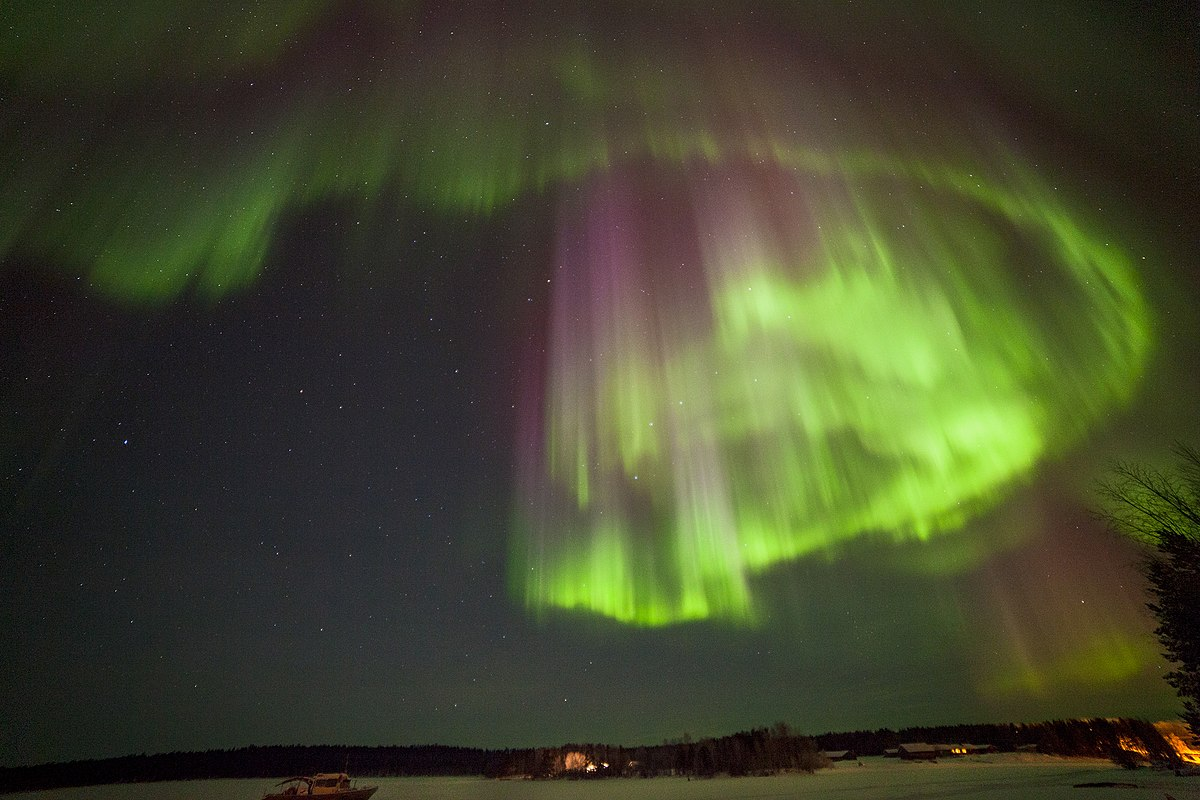
\includegraphics[width=.8\textwidth]{./2_natural_sky/aurora}
	\caption{Aurora borealis in the northern Finland. Credits: \href{https://commons.wikimedia.org/wiki/File:Aurora_Borealis_-_polar_lights_3.jpg}{Martincco}.\label{fig:aurora}}
\end{figure}

The occurrence and intensity of this phenomenon is strictly regulated by the solar activity, and an increase of auroral emission can be observed during solar storms or period of high activity. The phenomenon is observable only in polar regions, namely above \ang{80} of latitude (see \cite{eather1969latitudinal}) and for this reason it has a limited impact on the total optical sky background only in that geographic area. Nevertheless in case of intense solar activity like solar storms, aurorae can be observed at lower latitudes. Historical sources even report the sporadic observation of aurorae up to temperate latitudes.


\section{Atmospheric scattering}
Atmospheric scattering refers to the interaction of light with aerosol particles in the atmosphere. Unlike reflection or refraction, when a light beam get scattered its photons are deflected in random directions. In the Earth atmosphere the main aerosol particles are XXXXX.

\subsection{Scattering mechanisms}
There are two main scattering mechanism, depending on the size of the particle with respect to the wavelength of the incident radiation: Mie and Rayleigh scattering.

\paragraph{Mie scattering.}

\paragraph{Rayleigh scattering.}

\subsection{Effects on the sky brightness}
Every light source is responsible for a certain amount of light scattering. Depending on the site and the observation time, the effects of scattering on the total sky brightness can vary significantly.

\paragraph{Dark sites.} In a dark site most of the scattered light is produced by airglow, zodiacal light and the galactic background, i.e.\ the brightest ``direct'' light sources. According to \cite{leinert19981997} scattered light from the natural sources accounts for a brightness of the order of \num{e-8} to \SI{e-7}{erg\per\second \per\centi\metre\squared \per\steradian\per\angstrom}.

\paragraph{Light polluted sites.} Atmospheric light scattering is the main mechanism responsible for light pollution when far from the light source. Due to Earth curvature, geographic features and atmospheric extinction the direct light contribute to pollution only when very close to the light source. As reported in the chapter XX, brightness of scattered artificial light from a city varies with the population and the distance.

\paragraph{Scattered sunlight and moonlight.} Scattering is responsible for the twilight: even if the Sun is below the horizon some residual scattered light still brightens the sky. Conventionally astronomical twilight ends when the sun is \ang{18} below the horizon and other light sources, such as zodiacal light, becomes more relevant.

A similar effect is provided by scattered moonlight. Such light brightness depends on the lunar phase and on the distance between the Moon and the observing position in the sky. According to \cite{krisciunas1991model} and similar sources, in optical bands scattered moonlight can lead to an increase of the sky brightness of the order of \SI{5}{mag\per {arcsec}\squared}.

\bibliography{bibliography}
\bibliographystyle{alpha}

\end{document}